\documentclass[12pt]{article}\usepackage[]{graphicx}\usepackage[]{color}
%% maxwidth is the original width if it is less than linewidth
%% otherwise use linewidth (to make sure the graphics do not exceed the margin)
\makeatletter
\def\maxwidth{ %
  \ifdim\Gin@nat@width>\linewidth
    \linewidth
  \else
    \Gin@nat@width
  \fi
}
\makeatother

\definecolor{fgcolor}{rgb}{0.345, 0.345, 0.345}
\newcommand{\hlnum}[1]{\textcolor[rgb]{0.686,0.059,0.569}{#1}}%
\newcommand{\hlstr}[1]{\textcolor[rgb]{0.192,0.494,0.8}{#1}}%
\newcommand{\hlcom}[1]{\textcolor[rgb]{0.678,0.584,0.686}{\textit{#1}}}%
\newcommand{\hlopt}[1]{\textcolor[rgb]{0,0,0}{#1}}%
\newcommand{\hlstd}[1]{\textcolor[rgb]{0.345,0.345,0.345}{#1}}%
\newcommand{\hlkwa}[1]{\textcolor[rgb]{0.161,0.373,0.58}{\textbf{#1}}}%
\newcommand{\hlkwb}[1]{\textcolor[rgb]{0.69,0.353,0.396}{#1}}%
\newcommand{\hlkwc}[1]{\textcolor[rgb]{0.333,0.667,0.333}{#1}}%
\newcommand{\hlkwd}[1]{\textcolor[rgb]{0.737,0.353,0.396}{\textbf{#1}}}%

\usepackage{framed}
\makeatletter
\newenvironment{kframe}{%
 \def\at@end@of@kframe{}%
 \ifinner\ifhmode%
  \def\at@end@of@kframe{\end{minipage}}%
  \begin{minipage}{\columnwidth}%
 \fi\fi%
 \def\FrameCommand##1{\hskip\@totalleftmargin \hskip-\fboxsep
 \colorbox{shadecolor}{##1}\hskip-\fboxsep
     % There is no \\@totalrightmargin, so:
     \hskip-\linewidth \hskip-\@totalleftmargin \hskip\columnwidth}%
 \MakeFramed {\advance\hsize-\width
   \@totalleftmargin\z@ \linewidth\hsize
   \@setminipage}}%
 {\par\unskip\endMakeFramed%
 \at@end@of@kframe}
\makeatother

\definecolor{shadecolor}{rgb}{.97, .97, .97}
\definecolor{messagecolor}{rgb}{0, 0, 0}
\definecolor{warningcolor}{rgb}{1, 0, 1}
\definecolor{errorcolor}{rgb}{1, 0, 0}
\newenvironment{knitrout}{}{} % an empty environment to be redefined in TeX

\usepackage{alltt}
\usepackage{titlesec}
\usepackage{graphicx}
\usepackage{hyperref}
\hypersetup{
    bookmarks=true,         % show bookmarks bar?
    unicode=false,          % non-Latin characters in Acrobat’s bookmarks
    pdftoolbar=true,        % show Acrobat’s toolbar?
    pdfmenubar=true,        % show Acrobat’s menu?
    pdffitwindow=false,     % window fit to page when opened
    pdfstartview={FitH},    % fits the width of the page to the window
    pdftitle={Introduction to R},    % title
    pdfauthor={Thomas J. Leeper},     % author
    pdfsubject={Political Science},   % subject of the document
    pdfkeywords={R}, 		% list of keywords
    pdfnewwindow=true,      % links in new window
    colorlinks=false,       % false: boxed links; true: colored links
    pdfborder={0 0 0}
}
\usepackage{mdwlist}
\usepackage[top=1in, bottom=1in, left=1in, right=1in]{geometry}
\usepackage{natbib}
\bibpunct{(}{)}{;}{a}{}{,} %set in-line reference punctuation
\usepackage{setspace}
\setlength{\bibsep}{0.1in} %set spacing between references
\setlength{\bibhang}{.5in} %set hanging indent for references
\setlength{\parindent}{0.5in}

\title{Really Introductory Introduction to R}
\author{Thomas J. Leeper\\
Department of Government\\
London School of Economics and Political Science}
\IfFileExists{upquote.sty}{\usepackage{upquote}}{}
\begin{document}

\maketitle




{\abstract The purpose of this document is to provide a brief introduction to R, focused on the core code needed to load and analyze social scientific data. While numerous other resources exist online to facilitate learning R and to provide guidance on performing particular procedures, this document serves as a quick-start guide catered to the needs of students who are learning R for the first time in the context of a course that provides little technical instruction in programming. My aim in this document is to make learning R relatively more smooth so that you focus more of your attention on learning statistics and political science research methods and less on being frustrated with the particular software we are using to implement those ideas.\footnote{Some of this material is adapted from Teppei Yamamoto's (2009) ``Introduction to R'' Short Course. It is released without copyright, but citation is always appreciated.}}

\section{Why R?}\label{sec:intro}
R refers to a statistical computing environment and the programming language used therein. We use R in this course because it is free, open source, well-documented, involves a large community of active users, and, most importantly, because it provides nearly unlimited functionality that far exceeds that of all other statistical packages.

The major drawback of using R is that it is difficult for new users to learn. If you have no background in programming, the learning curve can be very steep. Prior experience with statistical theory is often not terribly helpful for actually implementing that theory in R. Prior experience with other statistical packages (Stata, SAS, SPSS, Matlab) is somewhat helpful and several texts have been written to help users of those packages transition to R. If you have prior experience with programming in other languages, learning R will be relatively straightforward; BASIC, C\#, PHP, Python, Javascript, etc. all share certain similarities with R.

A second challenge is that not a lot of effort has been put into making R user-friendly for those with no programming experience. It is a command-based program. There is almost nothing to ``point-and-click'' anywhere in R. You need to learn to program in order to even use R. When you do something wrong in R, it will give you an error message. These errors are typically cryptic and unhelpful. Trial-and-error, use of the online help files, and use of Google will all be necessary. Your instructor and TA should not be your first resources for problems with R. There is a wealth of information on the internet about R and you should plan on using your classmates as resources for troubleshooting. I am here to help you when you have exhausted these other resources. \textbf{I expect you to spend at least 20 minutes trying to solve a problem and have thoroughly read the relevant help files before emailing me.}

So why use R if it is so difficult to learn and so different other statistical packages that are also widely used and with which you might already be familiar? The payoff of learning can be substantial. Because R is a programming language, it allows you an incredible amount of flexibility for the manipulation of data, the creation of unique functions for analyzing and describing those data, and unparalleled functionality for the tabular and graphical presentation of data. For these reasons, R can actually be fun, once you get to know it. Being competent in R will make learning other programming languages and other statistical packages much easier --- skills that may prove useful and/or necessary in your future careers. And, once you know how to program and do statistical analysis, people will think you're really intelligent even if you are not, which has its advantages on the job market.

So, let's get started with R.

\section{Getting Started}
The first step is downloading and installing R. This is straightforward and instructions can be found on the R homepage \url{https://www.r-project.org}. On that package click ``CRAN'' on the left-hand side to find an appropriate download for your operating system. R runs on all major operating systems in effectively the exact same fashion (yet another advantage of R!). Once you have R installed, you can open it and you'll be presented with a command line. This is where you tell R what you want to do. Because you don't know how to program any R code yet, try using R as a calculator. The standard mathematical operators all work, and follow the `order of operations.' Here are some simple examples: 
\begin{knitrout}
\definecolor{shadecolor}{rgb}{0.969, 0.969, 0.969}\color{fgcolor}\begin{kframe}
\begin{alltt}
\hlnum{2}\hlopt{+}\hlnum{2}
\end{alltt}
\begin{verbatim}
## [1] 4
\end{verbatim}
\begin{alltt}
\hlnum{51}\hlopt{-}\hlnum{38}
\end{alltt}
\begin{verbatim}
## [1] 13
\end{verbatim}
\begin{alltt}
\hlstd{(}\hlnum{2}\hlopt{+}\hlnum{4}\hlstd{)}\hlopt{*}\hlnum{6}
\end{alltt}
\begin{verbatim}
## [1] 36
\end{verbatim}
\begin{alltt}
\hlnum{20}\hlopt{/}\hlnum{4}
\end{alltt}
\begin{verbatim}
## [1] 5
\end{verbatim}
\begin{alltt}
\hlnum{2}\hlopt{^}\hlnum{3}
\end{alltt}
\begin{verbatim}
## [1] 8
\end{verbatim}
\begin{alltt}
\hlkwd{sqrt}\hlstd{(}\hlnum{4}\hlstd{)}
\end{alltt}
\begin{verbatim}
## [1] 2
\end{verbatim}
\end{kframe}
\end{knitrout}

But, R is more than just a calculator (obviously!). To move away from using R as nothing more than a bloated calculator, we need to start doing some actual programming. But before we start writing more complex code, you'll probably want to move away from typing code directly into R and instead use another program to help you keep track of your code. There are a number of programs that can facilitate programming in R and dealing with its text and graphical outputs. First, you need a text editor to save the code you write. R doesn't automatically save the code that you tell it, so you'll save yourself a lot of time if you save all of your code in a separate program. You can use simple programs like Notepad, Wordpad, or even Word to do this, but better programs exist like Notepad++ (what I use), Emacs, Visual Studio, or RStudio.%\footnote{While I'd highly recommend you use a separate program to save your code, I cannot provide you any assistance with these other programs.}
\begin{itemize*}
\item Simple text editors: Notepad, TextPad, TextEdit, Wordpad (usually one or more of these is built-in with your computer's operating system)
\item Simple editor built in to R: \href{https://cran.r-project.org/web/packages/rite/index.html}{rite} (install and open with \texttt{install.packages("rite"); library("rite")}
\item Fancier text editors: \href{http://sciviews.org/Tinn-R/}{TINN-R}, \href{http://www.winedt.com/}{WinEdt}, \href{http://www.gnu.org/software/emacs/}{Emacs}, \href{http://aquamacs.org/}{Aquamacs}, \href{http://notepad-plus-plus.org/}{Notepad++}
\item Advanced front-ends for R: \href{http://rstudio.org/}{RStudio}, \href{http://www.revolutionanalytics.com/products/revolution-enterprise.php}{Revolution R}, \href{https://www.visualstudio.com/}{Visual Studio}
\item Graphical User Interface for R: \href{http://socserv.mcmaster.ca/jfox/Misc/Rcmdr/}{Rcmdr}
\end{itemize*}

If you save all of your code in one of these programs with a \texttt{.R} file extension, you should be able to completely reproduce your analysis simply by opening this file with R or copying and pasting the entirety of the code into R. This is helpful if you ask someone for help with your code because they can run all of your code and see where it may have had problems.

\subsection{Some General Notes Before Getting Started}

Some things to know about R and the R interpreter that you'll be interacting with:

\begin{itemize*}
\item R is basically a functional programming language with certain object-oriented capabilities. That means when we talk about particular statistics or procedures, we have to write code that tells R how to perform that statistical \emph{procedure} on a \emph{data object} and the function will generally return some new object. Usually, this looks something like \texttt{mean(x)}, where \texttt{mean()} is a procedure and \texttt{x} is an object (specifically, a vector of data points) and the result is a new object, which we can print to the console, save for later reuse, or simply abandon. When you first start working with R code, it can be hard to distinguish what text is a procedure from what text is the label for a data object, but over time this will get easier. If you use a text editor with syntax recognition, the text editor will highlight procedures (and sometimes objects) making the process of reading and writing code even easier.
\item R is case-sensitive. You need to type commands and variable names correctly or they will not work. As an example, \texttt{Mean()} does not mean \texttt{mean()}.
\item Arrow up and Arrow down on your keyboard cycle through previous commands you have entered. They do not scroll the screen up and down. Use your mouse scrollpad, Page Up and Page Down, or the scrollbar instead.
\item If you forget to put closing brackets on your commands, R will get confused and give you a \texttt{+} symbol instead of the usual \texttt{>} prompt. You can simply type the closing bracket in and the command will execute as if you typed it correctly the first time. This also means that R doesn't really recognize linebreaks. If you have a very long command (like for plots, which we'll talk about later), you may want to put the command on multiple lines so it is easier to read and R will have no problem with this, as long as you put the appropriate closing bracket at the end. If you use Mac OS or Linux OS, or some of the fancier text editors, closing brackets are often put in automatically as you type.
\end{itemize*}

\noindent Some general advice for when things eventually go wrong in R:

\begin{enumerate}
\item Don't panic!
\item Parsing errors versus syntax errors:
	\begin{itemize}
	\item Parsing errors mean you typed something wrong: \texttt{Error: unexpected ')' in "lm(y \textasciitilde)"}
	\item Syntax errors mean you typed correctly but R didn't understand: \texttt{Error in eval(expr, envir, enclos) : object 'y' not found}
	\end{itemize}
\item Google the error or warning
\item Use \href{http://stackoverflow.com/questions/tagged/r}{StackOverflow} to get help
\end{enumerate}



\subsection{Creating simple constants and vectors}
To do statistical analysis, we need to have data. R has various objects for storing different types of data. The simplest way to store data is in a \emph{constant}. A constant, to R, is just a number that is given a name. We use the \texttt{<-} to store something into a particular labeled object; we can also use \texttt{=} to do this; or \texttt{->} by reversing the argument:
\begin{knitrout}
\definecolor{shadecolor}{rgb}{0.969, 0.969, 0.969}\color{fgcolor}\begin{kframe}
\begin{alltt}
\hlstd{a}\hlkwb{<-}\hlnum{4}
\hlstd{a} \hlkwb{<-} \hlnum{4}
\hlcom{# 4->a # this works, too}
\hlstd{a}
\end{alltt}
\begin{verbatim}
## [1] 4
\end{verbatim}
\end{kframe}
\end{knitrout}
Here, we've created a constant called \texttt{a}, which has the value 4. R doesn't automatically display the value of \texttt{a} when we assign a value to it. To see the value of \texttt{a}, you need to simply type \texttt{a} and hit \texttt{<enter>}. We can store multiple constants, give new values to a constant we've already defined, and then conduct mathematical operations on those constants:
\begin{knitrout}
\definecolor{shadecolor}{rgb}{0.969, 0.969, 0.969}\color{fgcolor}\begin{kframe}
\begin{alltt}
\hlstd{a} \hlkwb{<-} \hlnum{4}
\hlstd{a} \hlkwb{<-} \hlnum{6}
\hlstd{a}
\end{alltt}
\begin{verbatim}
## [1] 6
\end{verbatim}
\begin{alltt}
\hlstd{b} \hlkwb{<-} \hlnum{3}
\hlstd{b}\hlopt{+}\hlnum{2}
\end{alltt}
\begin{verbatim}
## [1] 5
\end{verbatim}
\begin{alltt}
\hlstd{b}\hlopt{*}\hlstd{a}
\end{alltt}
\begin{verbatim}
## [1] 18
\end{verbatim}
\end{kframe}
\end{knitrout}
Note that $b*a=18$ in the code above, even though we calculated \texttt{b+2} in the line directly above that calculation. You have to store a result as a constant to be able to use that result later.

Storing all of our data as individual constants, isn't very efficient, though. Let's say we want to collect a piece of data for a number of units (e.g., people in this class). We can store a set of data points as a \emph{vector} in R using the \texttt{c()} command. Vectors can have any length and we can perform mathematical operations on vectors.

\begin{knitrout}
\definecolor{shadecolor}{rgb}{0.969, 0.969, 0.969}\color{fgcolor}\begin{kframe}
\begin{alltt}
\hlstd{a} \hlkwb{<-} \hlkwd{c}\hlstd{(}\hlnum{1}\hlstd{,}\hlnum{2}\hlstd{,}\hlnum{3}\hlstd{,}\hlnum{4}\hlstd{,}\hlnum{5}\hlstd{,}\hlnum{6}\hlstd{,}\hlnum{7}\hlstd{,}\hlnum{8}\hlstd{,}\hlnum{9}\hlstd{,}\hlnum{10}\hlstd{)}
\hlstd{a}
\end{alltt}
\begin{verbatim}
##  [1]  1  2  3  4  5  6  7  8  9 10
\end{verbatim}
\begin{alltt}
\hlstd{a}\hlopt{*}\hlnum{2}
\end{alltt}
\begin{verbatim}
##  [1]  2  4  6  8 10 12 14 16 18 20
\end{verbatim}
\begin{alltt}
\hlstd{b} \hlkwb{<-} \hlstd{a}
\hlstd{b}
\end{alltt}
\begin{verbatim}
##  [1]  1  2  3  4  5  6  7  8  9 10
\end{verbatim}
\end{kframe}
\end{knitrout}

You can also create a sequence of numbers using \texttt{seq()} or just the \texttt{:}.
\begin{knitrout}
\definecolor{shadecolor}{rgb}{0.969, 0.969, 0.969}\color{fgcolor}\begin{kframe}
\begin{alltt}
\hlstd{a} \hlkwb{<-} \hlkwd{seq}\hlstd{(}\hlnum{1}\hlopt{:}\hlnum{10}\hlstd{)}
\hlstd{a}
\end{alltt}
\begin{verbatim}
##  [1]  1  2  3  4  5  6  7  8  9 10
\end{verbatim}
\begin{alltt}
\hlstd{b} \hlkwb{<-} \hlnum{1}\hlopt{:}\hlnum{10}
\hlstd{b}
\end{alltt}
\begin{verbatim}
##  [1]  1  2  3  4  5  6  7  8  9 10
\end{verbatim}
\end{kframe}
\end{knitrout}

This is especially helpful if we want to calculate any basic statistics on a particular vector of data (what we might, in social science language, call a variable). Let's imagine for instance that we collect a number of 2-dice rolls and record the sum in a vector called dice. We can then find out a number of pieces of information about this set of rolls.

\begin{knitrout}
\definecolor{shadecolor}{rgb}{0.969, 0.969, 0.969}\color{fgcolor}\begin{kframe}
\begin{alltt}
\hlstd{dice} \hlkwb{<-} \hlkwd{c}\hlstd{(}\hlnum{2}\hlstd{,}\hlnum{2}\hlstd{,}\hlnum{3}\hlstd{,}\hlnum{4}\hlstd{,}\hlnum{4}\hlstd{,}\hlnum{5}\hlstd{,}\hlnum{5}\hlstd{,}\hlnum{5}\hlstd{,}\hlnum{5}\hlstd{,}\hlnum{5}\hlstd{,}\hlnum{6}\hlstd{,}\hlnum{6}\hlstd{,}\hlnum{7}\hlstd{,}\hlnum{7}\hlstd{,}\hlnum{7}\hlstd{,}\hlnum{7}\hlstd{,}\hlnum{8}\hlstd{,}\hlnum{9}\hlstd{,}\hlnum{10}\hlstd{,}\hlnum{11}\hlstd{)}
\hlkwd{table}\hlstd{(dice)} \hlcom{#a simple tabulation of how many of each value are in the vector}
\end{alltt}
\begin{verbatim}
## dice
##  2  3  4  5  6  7  8  9 10 11 
##  2  1  2  5  2  4  1  1  1  1
\end{verbatim}
\begin{alltt}
\hlkwd{fivenum}\hlstd{(dice)} \hlcom{# the five number summary (min, Q1, median, Q3, max)}
\end{alltt}
\begin{verbatim}
## [1]  2.0  4.5  5.5  7.0 11.0
\end{verbatim}
\begin{alltt}
\hlkwd{quantile}\hlstd{(dice,} \hlkwd{c}\hlstd{(}\hlnum{0.1}\hlstd{,}\hlnum{0.2}\hlstd{,}\hlnum{0.6}\hlstd{,}\hlnum{0.8}\hlstd{))} \hlcom{# arbitrary quantiles}
\end{alltt}
\begin{verbatim}
## 10% 20% 60% 80% 
## 2.9 4.0 6.4 7.2
\end{verbatim}
\begin{alltt}
\hlkwd{summary}\hlstd{(dice)} \hlcom{# a set of basic univariate statistics for the vector}
\end{alltt}
\begin{verbatim}
##    Min. 1st Qu.  Median    Mean 3rd Qu.    Max. 
##    2.00    4.75    5.50    5.90    7.00   11.00
\end{verbatim}
\end{kframe}
\end{knitrout}

Note we can also obtain these summary values individually.
\begin{knitrout}
\definecolor{shadecolor}{rgb}{0.969, 0.969, 0.969}\color{fgcolor}\begin{kframe}
\begin{alltt}
\hlstd{dice} \hlkwb{<-} \hlkwd{c}\hlstd{(}\hlnum{2}\hlstd{,}\hlnum{2}\hlstd{,}\hlnum{3}\hlstd{,}\hlnum{4}\hlstd{,}\hlnum{4}\hlstd{,}\hlnum{5}\hlstd{,}\hlnum{5}\hlstd{,}\hlnum{5}\hlstd{,}\hlnum{5}\hlstd{,}\hlnum{5}\hlstd{,}\hlnum{6}\hlstd{,}\hlnum{6}\hlstd{,}\hlnum{7}\hlstd{,}\hlnum{7}\hlstd{,}\hlnum{7}\hlstd{,}\hlnum{7}\hlstd{,}\hlnum{8}\hlstd{,}\hlnum{9}\hlstd{,}\hlnum{10}\hlstd{,}\hlnum{11}\hlstd{)}
\hlkwd{length}\hlstd{(dice)} \hlcom{#how many observations are there?}
\end{alltt}
\begin{verbatim}
## [1] 20
\end{verbatim}
\begin{alltt}
\hlkwd{min}\hlstd{(dice)} \hlcom{#minimum}
\end{alltt}
\begin{verbatim}
## [1] 2
\end{verbatim}
\begin{alltt}
\hlkwd{median}\hlstd{(dice)} \hlcom{#median}
\end{alltt}
\begin{verbatim}
## [1] 5.5
\end{verbatim}
\begin{alltt}
\hlkwd{max}\hlstd{(dice)} \hlcom{#maximum}
\end{alltt}
\begin{verbatim}
## [1] 11
\end{verbatim}
\begin{alltt}
\hlkwd{max}\hlstd{(dice)}\hlopt{-}\hlkwd{min}\hlstd{(dice)} \hlcom{#range}
\end{alltt}
\begin{verbatim}
## [1] 9
\end{verbatim}
\begin{alltt}
\hlkwd{sum}\hlstd{(dice)}
\end{alltt}
\begin{verbatim}
## [1] 118
\end{verbatim}
\begin{alltt}
\hlkwd{sum}\hlstd{(dice)}\hlopt{/}\hlkwd{length}\hlstd{(dice)}
\end{alltt}
\begin{verbatim}
## [1] 5.9
\end{verbatim}
\begin{alltt}
\hlkwd{mean}\hlstd{(dice)} \hlcom{#mean}
\end{alltt}
\begin{verbatim}
## [1] 5.9
\end{verbatim}
\begin{alltt}
\hlstd{v} \hlkwb{<-} \hlkwd{var}\hlstd{(dice)} \hlcom{#variance}
\hlstd{v}
\end{alltt}
\begin{verbatim}
## [1] 5.884211
\end{verbatim}
\begin{alltt}
\hlkwd{sqrt}\hlstd{(v)} \hlcom{#standard deviation}
\end{alltt}
\begin{verbatim}
## [1] 2.425739
\end{verbatim}
\begin{alltt}
\hlkwd{sd}\hlstd{(dice)} \hlcom{#easier way of getting standard deviation}
\end{alltt}
\begin{verbatim}
## [1] 2.425739
\end{verbatim}
\end{kframe}
\end{knitrout}

One thing that can be initially confusing for new users of R is exactly what is happening when you type in a given command. R does not solve mathematical equations. Instead, like any programming language, it performs a set of procedures in a specific order on a particular data object (i.e., it performs an algorithm). What does an algorithm look like and why does it matter? To use R effectively, one needs to understand what it is doing and how to think in algorithms rather than equations. Think about the formula for the mean of a set of data (like our dice roll data). The mathematical equation is $\bar{x}=\Sigma x_{i} / n$. This translates into an R algorithm like the following:
\begin{knitrout}
\definecolor{shadecolor}{rgb}{0.969, 0.969, 0.969}\color{fgcolor}\begin{kframe}
\begin{alltt}
\hlstd{dice} \hlkwb{<-} \hlkwd{c}\hlstd{(}\hlnum{2}\hlstd{,}\hlnum{2}\hlstd{,}\hlnum{3}\hlstd{,}\hlnum{4}\hlstd{,}\hlnum{4}\hlstd{,}\hlnum{5}\hlstd{,}\hlnum{5}\hlstd{,}\hlnum{5}\hlstd{,}\hlnum{5}\hlstd{,}\hlnum{5}\hlstd{,}\hlnum{6}\hlstd{,}\hlnum{6}\hlstd{,}\hlnum{7}\hlstd{,}\hlnum{7}\hlstd{,}\hlnum{7}\hlstd{,}\hlnum{7}\hlstd{,}\hlnum{8}\hlstd{,}\hlnum{9}\hlstd{,}\hlnum{10}\hlstd{,}\hlnum{11}\hlstd{)}
\hlstd{s} \hlkwb{<-} \hlnum{2}\hlopt{+}\hlnum{2}\hlopt{+}\hlnum{3}\hlopt{+}\hlnum{4}\hlopt{+}\hlnum{4}\hlopt{+}\hlnum{5}\hlopt{+}\hlnum{5}\hlopt{+}\hlnum{5}\hlopt{+}\hlnum{5}\hlopt{+}\hlnum{5}\hlopt{+}\hlnum{6}\hlopt{+}\hlnum{6}\hlopt{+}\hlnum{7}\hlopt{+}\hlnum{7}\hlopt{+}\hlnum{7}\hlopt{+}\hlnum{7}\hlopt{+}\hlnum{8}\hlopt{+}\hlnum{9}\hlopt{+}\hlnum{10}\hlopt{+}\hlnum{11}
\hlstd{s}
\end{alltt}
\begin{verbatim}
## [1] 118
\end{verbatim}
\begin{alltt}
\hlstd{len} \hlkwb{<-} \hlkwd{length}\hlstd{(dice)}
\hlstd{len}
\end{alltt}
\begin{verbatim}
## [1] 20
\end{verbatim}
\begin{alltt}
\hlstd{m} \hlkwb{<-} \hlstd{s}\hlopt{/}\hlstd{len}
\hlstd{m}
\end{alltt}
\begin{verbatim}
## [1] 5.9
\end{verbatim}
\end{kframe}
\end{knitrout}

As we can see, the result is the same as using R's built-in \texttt{mean()} function. We could attempt something similar by converting the equation for variance ($Var[x]=\Sigma (x_{i} - \bar{x})^2 / (n-1)$) into an algorithm (the first four steps of which are the same as calculating the mean):
\begin{enumerate*}
\item Load the vector of all $x_i$, called \emph{data}
\item Sum all $x_i$, store this result as \emph{sum}
\item Count the number of $x_i$, store this as \emph{length}
\item Divide \emph{sum} by \emph{length}, store this as \emph{mean}
\item Create a new vector, where each entry in the vector is the difference between each $x_i$ in \emph{data} and mean of all $x_i$ (\emph{mean}),  store as \emph{deviations}
\item Create a new vector, where each entry is the square of the entry in \emph{deviations}, store as \emph{squares}
\item Sum all values in \emph{squares}, store as \emph{sumsquares}
\item Divide \emph{sumsquares} by one less than \emph{length}, store as \emph{variance}
\end{enumerate*}
We can then write that algorithm in R:
\begin{knitrout}
\definecolor{shadecolor}{rgb}{0.969, 0.969, 0.969}\color{fgcolor}\begin{kframe}
\begin{alltt}
\hlstd{dice} \hlkwb{<-} \hlkwd{c}\hlstd{(}\hlnum{2}\hlstd{,}\hlnum{2}\hlstd{,}\hlnum{3}\hlstd{,}\hlnum{4}\hlstd{,}\hlnum{4}\hlstd{,}\hlnum{5}\hlstd{,}\hlnum{5}\hlstd{,}\hlnum{5}\hlstd{,}\hlnum{5}\hlstd{,}\hlnum{5}\hlstd{,}\hlnum{6}\hlstd{,}\hlnum{6}\hlstd{,}\hlnum{7}\hlstd{,}\hlnum{7}\hlstd{,}\hlnum{7}\hlstd{,}\hlnum{7}\hlstd{,}\hlnum{8}\hlstd{,}\hlnum{9}\hlstd{,}\hlnum{10}\hlstd{,}\hlnum{11}\hlstd{)}
\hlstd{s} \hlkwb{<-} \hlkwd{sum}\hlstd{(dice)}
\hlstd{len} \hlkwb{<-} \hlkwd{length}\hlstd{(dice)}
\hlstd{m} \hlkwb{<-} \hlstd{s}\hlopt{/}\hlstd{len}
\hlstd{deviations} \hlkwb{<-} \hlstd{dice}\hlopt{-}\hlstd{m}
\hlstd{squares} \hlkwb{<-} \hlstd{deviations}\hlopt{^}\hlnum{2}
\hlstd{sumsquares} \hlkwb{<-} \hlkwd{sum}\hlstd{(squares)}
\hlstd{v} \hlkwb{<-} \hlstd{sumsquares}\hlopt{/}\hlstd{(len}\hlopt{-}\hlnum{1}\hlstd{)}
\hlstd{v}
\end{alltt}
\begin{verbatim}
## [1] 5.884211
\end{verbatim}
\begin{alltt}
\hlkwd{sqrt}\hlstd{(v)}
\end{alltt}
\begin{verbatim}
## [1] 2.425739
\end{verbatim}
\end{kframe}
\end{knitrout}

As we can see, our mathematical equation for variance is easily converted to an algorithm that we can then write in R code. While the \texttt{var()} command is short and simple, it reflects all of this underlying code. While we can rely on these built-in functions, it is important to keep in mind what is happening behind the scenes. Thinking like a computer programmer rather than a math student will greatly facilitate your transition to R.

Two additional important tips here. First, you can use the \texttt{round()} command to round a given value to a specified number of decimal places. Second, you can nest commands inside of one another rather than produce a constant that you'll only use one time (e.g., to calculate the standard deviation we can create a constant that stores the variance and take the square root thereof OR we can simply take the square root of the variance directly).
\begin{knitrout}
\definecolor{shadecolor}{rgb}{0.969, 0.969, 0.969}\color{fgcolor}\begin{kframe}
\begin{alltt}
\hlkwd{round}\hlstd{(}\hlkwd{mean}\hlstd{(dice),}\hlnum{2}\hlstd{)}
\end{alltt}
\begin{verbatim}
## [1] 5.9
\end{verbatim}
\begin{alltt}
\hlkwd{round}\hlstd{(}\hlkwd{sqrt}\hlstd{(}\hlkwd{var}\hlstd{(dice)),}\hlnum{2}\hlstd{)}
\end{alltt}
\begin{verbatim}
## [1] 2.43
\end{verbatim}
\end{kframe}
\end{knitrout}

We can also extract one or more observations from a vector. For instance, if we wanted to know the value of the 1st through 3rd rolls, or just the value of the 7th roll:
\begin{knitrout}
\definecolor{shadecolor}{rgb}{0.969, 0.969, 0.969}\color{fgcolor}\begin{kframe}
\begin{alltt}
\hlstd{dice} \hlkwb{<-} \hlkwd{c}\hlstd{(}\hlnum{2}\hlstd{,}\hlnum{2}\hlstd{,}\hlnum{3}\hlstd{,}\hlnum{4}\hlstd{,}\hlnum{4}\hlstd{,}\hlnum{5}\hlstd{,}\hlnum{5}\hlstd{,}\hlnum{5}\hlstd{,}\hlnum{5}\hlstd{,}\hlnum{5}\hlstd{,}\hlnum{6}\hlstd{,}\hlnum{6}\hlstd{,}\hlnum{7}\hlstd{,}\hlnum{7}\hlstd{,}\hlnum{7}\hlstd{,}\hlnum{7}\hlstd{,}\hlnum{8}\hlstd{,}\hlnum{9}\hlstd{,}\hlnum{10}\hlstd{,}\hlnum{11}\hlstd{)}
\hlstd{dice[}\hlnum{1}\hlopt{:}\hlnum{3}\hlstd{]}
\end{alltt}
\begin{verbatim}
## [1] 2 2 3
\end{verbatim}
\begin{alltt}
\hlstd{dice[}\hlnum{7}\hlstd{]}
\end{alltt}
\begin{verbatim}
## [1] 5
\end{verbatim}
\end{kframe}
\end{knitrout}
We'll discuss more about extracting particular observations in a moment. Clearly, though, conducting simple analyses in R is pretty straightfoward. Most of the commands are semantic --- that is, the command to obtain a particular statistic is intuitive. This is generally the case, but can get confusing once we move into more advanced statistics. Using comments in your R programming will therefore be vital to you and I both understanding what you're trying to do with a given piece of code. The pound sign (\#) can be used to create comments in the code, which can be helpful when you have to do complex things in your code and you want to remind yourself (or me) what you're trying to do with each bit of code. They can be included at the end of a line of code or simply on their own. Just start the line with a pound sign and then continue with code on the next line.

Now let's work with two variables. Let's try comparing two sets of dice rolls, by looking at their means, variances, and the correlation between the two sets of rolls.
\begin{knitrout}
\definecolor{shadecolor}{rgb}{0.969, 0.969, 0.969}\color{fgcolor}\begin{kframe}
\begin{alltt}
\hlstd{dice1} \hlkwb{<-} \hlkwd{c}\hlstd{(}\hlnum{7}\hlstd{,}\hlnum{7}\hlstd{,}\hlnum{4}\hlstd{,}\hlnum{5}\hlstd{,}\hlnum{3}\hlstd{,}\hlnum{6}\hlstd{,}\hlnum{8}\hlstd{,}\hlnum{2}\hlstd{,}\hlnum{12}\hlstd{,}\hlnum{10}\hlstd{)}
\hlstd{dice2} \hlkwb{<-} \hlkwd{c}\hlstd{(}\hlnum{8}\hlstd{,}\hlnum{4}\hlstd{,}\hlnum{7}\hlstd{,}\hlnum{7}\hlstd{,}\hlnum{7}\hlstd{,}\hlnum{7}\hlstd{,}\hlnum{6}\hlstd{,}\hlnum{6}\hlstd{,}\hlnum{3}\hlstd{,}\hlnum{4}\hlstd{)}
\hlkwd{mean}\hlstd{(dice1)}
\end{alltt}
\begin{verbatim}
## [1] 6.4
\end{verbatim}
\begin{alltt}
\hlkwd{sd}\hlstd{(dice1)}
\end{alltt}
\begin{verbatim}
## [1] 3.098387
\end{verbatim}
\begin{alltt}
\hlkwd{mean}\hlstd{(dice2)}
\end{alltt}
\begin{verbatim}
## [1] 5.9
\end{verbatim}
\begin{alltt}
\hlkwd{sd}\hlstd{(dice2)}
\end{alltt}
\begin{verbatim}
## [1] 1.66333
\end{verbatim}
\begin{alltt}
\hlkwd{cor}\hlstd{(dice1,dice2)}
\end{alltt}
\begin{verbatim}
## [1] -0.6812877
\end{verbatim}
\end{kframe}
\end{knitrout}

\subsection{Creating matrices and data.frames}

We could also represent these data a different way. Rather than having two vectors, we could ``column bind'' them (using the \texttt{cbind()} command) into a \emph{matrix}, which we can also call whatever we want.
\begin{knitrout}
\definecolor{shadecolor}{rgb}{0.969, 0.969, 0.969}\color{fgcolor}\begin{kframe}
\begin{alltt}
\hlstd{dice1} \hlkwb{<-} \hlkwd{c}\hlstd{(}\hlnum{7}\hlstd{,}\hlnum{7}\hlstd{,}\hlnum{4}\hlstd{,}\hlnum{5}\hlstd{,}\hlnum{3}\hlstd{,}\hlnum{6}\hlstd{,}\hlnum{8}\hlstd{,}\hlnum{2}\hlstd{,}\hlnum{12}\hlstd{,}\hlnum{10}\hlstd{)}
\hlstd{dice2} \hlkwb{<-} \hlkwd{c}\hlstd{(}\hlnum{8}\hlstd{,}\hlnum{4}\hlstd{,}\hlnum{7}\hlstd{,}\hlnum{7}\hlstd{,}\hlnum{7}\hlstd{,}\hlnum{7}\hlstd{,}\hlnum{6}\hlstd{,}\hlnum{6}\hlstd{,}\hlnum{3}\hlstd{,}\hlnum{4}\hlstd{)}
\hlstd{dice} \hlkwb{<-} \hlkwd{c}\hlstd{(dice1,dice2)}
\hlstd{set} \hlkwb{<-} \hlkwd{c}\hlstd{(}\hlnum{1}\hlstd{,}\hlnum{1}\hlstd{,}\hlnum{1}\hlstd{,}\hlnum{1}\hlstd{,}\hlnum{1}\hlstd{,}\hlnum{1}\hlstd{,}\hlnum{1}\hlstd{,}\hlnum{1}\hlstd{,}\hlnum{1}\hlstd{,}\hlnum{1}\hlstd{,}\hlnum{2}\hlstd{,}\hlnum{2}\hlstd{,}\hlnum{2}\hlstd{,}\hlnum{2}\hlstd{,}\hlnum{2}\hlstd{,}\hlnum{2}\hlstd{,}\hlnum{2}\hlstd{,}\hlnum{2}\hlstd{,}\hlnum{2}\hlstd{,}\hlnum{2}\hlstd{)}
\hlstd{dice.mat} \hlkwb{<-} \hlkwd{cbind}\hlstd{(set,dice)}
\hlstd{dice.mat}
\end{alltt}
\begin{verbatim}
##       set dice
##  [1,]   1    7
##  [2,]   1    7
##  [3,]   1    4
##  [4,]   1    5
##  [5,]   1    3
##  [6,]   1    6
##  [7,]   1    8
##  [8,]   1    2
##  [9,]   1   12
## [10,]   1   10
## [11,]   2    8
## [12,]   2    4
## [13,]   2    7
## [14,]   2    7
## [15,]   2    7
## [16,]   2    7
## [17,]   2    6
## [18,]   2    6
## [19,]   2    3
## [20,]   2    4
\end{verbatim}
\end{kframe}
\end{knitrout}

We can also use the corresponding \texttt{rbind()} to ``row bind'' two or more vectors, which has the same effect as \texttt{cbind()}, but treats each vector as a row/observation. The \texttt{t()} command transposes a matrix. If we apply this function to our original matrix (that we constructed using \texttt{cbind()}), we will obtain the second matrix we constructed (using \texttt{rbind()}).
\begin{knitrout}
\definecolor{shadecolor}{rgb}{0.969, 0.969, 0.969}\color{fgcolor}\begin{kframe}
\begin{alltt}
\hlkwd{rbind}\hlstd{(set,dice)}
\end{alltt}
\begin{verbatim}
##      [,1] [,2] [,3] [,4] [,5] [,6] [,7] [,8] [,9] [,10] [,11] [,12] [,13]
## set     1    1    1    1    1    1    1    1    1     1     2     2     2
## dice    7    7    4    5    3    6    8    2   12    10     8     4     7
##      [,14] [,15] [,16] [,17] [,18] [,19] [,20]
## set      2     2     2     2     2     2     2
## dice     7     7     7     6     6     3     4
\end{verbatim}
\begin{alltt}
\hlkwd{t}\hlstd{(dice.mat)}
\end{alltt}
\begin{verbatim}
##      [,1] [,2] [,3] [,4] [,5] [,6] [,7] [,8] [,9] [,10] [,11] [,12] [,13]
## set     1    1    1    1    1    1    1    1    1     1     2     2     2
## dice    7    7    4    5    3    6    8    2   12    10     8     4     7
##      [,14] [,15] [,16] [,17] [,18] [,19] [,20]
## set      2     2     2     2     2     2     2
## dice     7     7     7     6     6     3     4
\end{verbatim}
\end{kframe}
\end{knitrout}

Here, we created our vectors from above, but then combined them into a single vector using the \texttt{c()} command. We then created a separate vector called \texttt{set} into which we stored the identifier for whether the observation came from our first or second set of rolls. We then bound these two vectors together into a matrix called \texttt{dice.mat}, which has dimensions 20 x 2. Now this is starting to look like a traditional rectangular dataset where each observation is represented as a row and each variable is a column. We can look at the dimensions of the new matrix, including its number of columns and number of rows and use that information to extract particular values (or sets of values) from the matrix. We can extract a particular observation (e.g., observation 5), a particular variable (e.g., the second variable), or the observation for a given variable (e.g., the value of the roll for our fifth roll) just as we did with vectors, but now our syntax reflects that row and column position, as follows:
\begin{knitrout}
\definecolor{shadecolor}{rgb}{0.969, 0.969, 0.969}\color{fgcolor}\begin{kframe}
\begin{alltt}
\hlkwd{ncol}\hlstd{(dice.mat)}
\end{alltt}
\begin{verbatim}
## [1] 2
\end{verbatim}
\begin{alltt}
\hlkwd{nrow}\hlstd{(dice.mat)}
\end{alltt}
\begin{verbatim}
## [1] 20
\end{verbatim}
\begin{alltt}
\hlkwd{dim}\hlstd{(dice.mat)} \hlcom{#obtain both dimensions}
\end{alltt}
\begin{verbatim}
## [1] 20  2
\end{verbatim}
\begin{alltt}
\hlstd{dice.mat[}\hlnum{5}\hlstd{,]}
\end{alltt}
\begin{verbatim}
##  set dice 
##    1    3
\end{verbatim}
\begin{alltt}
\hlstd{dice.mat[,}\hlnum{2}\hlstd{]}
\end{alltt}
\begin{verbatim}
##  [1]  7  7  4  5  3  6  8  2 12 10  8  4  7  7  7  7  6  6  3  4
\end{verbatim}
\begin{alltt}
\hlstd{dice.mat[}\hlnum{5}\hlstd{,}\hlnum{2}\hlstd{]}
\end{alltt}
\begin{verbatim}
## dice 
##    3
\end{verbatim}
\end{kframe}
\end{knitrout}

We could continue to bind vectors to this matrix. For example, we could bind a vector to the matrix that identifies the color the dice we rolled. Here we'll be dealing with a vector of \emph{strings}, which we cannot perform statistical or mathematical operations, but that we often find in real world data.
\begin{knitrout}
\definecolor{shadecolor}{rgb}{0.969, 0.969, 0.969}\color{fgcolor}\begin{kframe}
\begin{alltt}
\hlstd{color} \hlkwb{<-} \hlkwd{c}\hlstd{(}\hlstr{"red"}\hlstd{,}\hlstr{"red"}\hlstd{,}\hlstr{"blue"}\hlstd{,}\hlstr{"yellow"}\hlstd{,}\hlstr{"blue"}\hlstd{,}\hlstr{"red"}\hlstd{,}\hlstr{"red"}\hlstd{,}
        \hlstr{"blue"}\hlstd{,}\hlstr{"yellow"}\hlstd{,}\hlstr{"blue"}\hlstd{,}\hlstr{"red"}\hlstd{,}\hlstr{"red"}\hlstd{,}\hlstr{"blue"}\hlstd{,}\hlstr{"yellow"}\hlstd{,}
        \hlstr{"blue"}\hlstd{,}\hlstr{"red"}\hlstd{,}\hlstr{"red"}\hlstd{,}\hlstr{"blue"}\hlstd{,}\hlstr{"yellow"}\hlstd{,}\hlstr{"blue"}\hlstd{)}
\hlstd{dice.mat2} \hlkwb{<-} \hlkwd{cbind}\hlstd{(dice.mat,color)}
\hlstd{dice.mat2}
\end{alltt}
\begin{verbatim}
##       set dice color   
##  [1,] "1" "7"  "red"   
##  [2,] "1" "7"  "red"   
##  [3,] "1" "4"  "blue"  
##  [4,] "1" "5"  "yellow"
##  [5,] "1" "3"  "blue"  
##  [6,] "1" "6"  "red"   
##  [7,] "1" "8"  "red"   
##  [8,] "1" "2"  "blue"  
##  [9,] "1" "12" "yellow"
## [10,] "1" "10" "blue"  
## [11,] "2" "8"  "red"   
## [12,] "2" "4"  "red"   
## [13,] "2" "7"  "blue"  
## [14,] "2" "7"  "yellow"
## [15,] "2" "7"  "blue"  
## [16,] "2" "7"  "red"   
## [17,] "2" "6"  "red"   
## [18,] "2" "6"  "blue"  
## [19,] "2" "3"  "yellow"
## [20,] "2" "4"  "blue"
\end{verbatim}
\end{kframe}
\end{knitrout}

We can also transform this matrix into a different type of R object called a \emph{data.frame}. Matrices and data.frames have some similar properties, but also differences that you will learn over the course of this course. Importantly, most data that we read in from an outside file (as opposed to typing in ourselves) will be in the form of a data.frame. But, we can also transform our matrix into a data.frame. If you want to know whether something is a matrix or a data.frame, you can also test it using an \texttt{is.matrix()} or \texttt{is.data.frame()} command.
\begin{knitrout}
\definecolor{shadecolor}{rgb}{0.969, 0.969, 0.969}\color{fgcolor}\begin{kframe}
\begin{alltt}
\hlstd{data.frame} \hlkwb{<-} \hlkwd{as.data.frame}\hlstd{(dice.mat2)}
\hlkwd{is.data.frame}\hlstd{(data.frame)}
\end{alltt}
\begin{verbatim}
## [1] TRUE
\end{verbatim}
\begin{alltt}
\hlkwd{is.matrix}\hlstd{(data.frame)}
\end{alltt}
\begin{verbatim}
## [1] FALSE
\end{verbatim}
\begin{alltt}
\hlkwd{is.data.frame}\hlstd{(dice.mat2)}
\end{alltt}
\begin{verbatim}
## [1] FALSE
\end{verbatim}
\begin{alltt}
\hlkwd{is.matrix}\hlstd{(dice.mat2)}
\end{alltt}
\begin{verbatim}
## [1] TRUE
\end{verbatim}
\end{kframe}
\end{knitrout}

One of the key advantages of data.frames is that we can refer to columns of the data.frame by their variable names, as opposed to their position number (as we have to do with matrices). We can find these names using the \texttt{names()} command and isolate a particular column of the matrix by using the dollar sign operator. Note that this produces the same result as using the brackets to identify the particular column (as we did above with our matrix).
\begin{knitrout}
\definecolor{shadecolor}{rgb}{0.969, 0.969, 0.969}\color{fgcolor}\begin{kframe}
\begin{alltt}
\hlkwd{names}\hlstd{(data.frame)}
\end{alltt}
\begin{verbatim}
## [1] "set"   "dice"  "color"
\end{verbatim}
\begin{alltt}
\hlstd{data.frame}\hlopt{$}\hlstd{color}
\end{alltt}
\begin{verbatim}
##  [1] red    red    blue   yellow blue   red    red    blue   yellow blue  
## [11] red    red    blue   yellow blue   red    red    blue   yellow blue  
## Levels: blue red yellow
\end{verbatim}
\begin{alltt}
\hlstd{data.frame[,}\hlnum{3}\hlstd{]}
\end{alltt}
\begin{verbatim}
##  [1] red    red    blue   yellow blue   red    red    blue   yellow blue  
## [11] red    red    blue   yellow blue   red    red    blue   yellow blue  
## Levels: blue red yellow
\end{verbatim}
\end{kframe}
\end{knitrout}

We can also extract a column or row from a data.frame and turn it into a vector. We might want to do this if we plan on transforming the data in some way and saving that transformed data for later use. We could also add that new vector back into the data.frame under a new name. The vector and column in the data.frame will have the same properties, but changing one has no effect on the other. This aspect can sometimes get confusing, especially once you start working with data that contains many variables. You can have a column in a data.frame and a separate vector that have the same name. To work with the vector simply use the name, to use the column in the data.frame, you have to use the \texttt{\$} operator.
\begin{knitrout}
\definecolor{shadecolor}{rgb}{0.969, 0.969, 0.969}\color{fgcolor}\begin{kframe}
\begin{alltt}
\hlstd{df} \hlkwb{<-} \hlkwd{as.data.frame}\hlstd{(dice.mat)}
\hlstd{df}\hlopt{$}\hlstd{dice}
\end{alltt}
\begin{verbatim}
##  [1]  7  7  4  5  3  6  8  2 12 10  8  4  7  7  7  7  6  6  3  4
\end{verbatim}
\begin{alltt}
\hlstd{half} \hlkwb{<-} \hlstd{df}\hlopt{$}\hlstd{dice}\hlopt{+}\hlnum{1}
\hlstd{df}\hlopt{$}\hlstd{half} \hlkwb{<-} \hlstd{half}
\hlkwd{summary}\hlstd{(half)}
\end{alltt}
\begin{verbatim}
##    Min. 1st Qu.  Median    Mean 3rd Qu.    Max. 
##    3.00    5.00    7.50    7.15    8.00   13.00
\end{verbatim}
\begin{alltt}
\hlkwd{summary}\hlstd{(df}\hlopt{$}\hlstd{half)}
\end{alltt}
\begin{verbatim}
##    Min. 1st Qu.  Median    Mean 3rd Qu.    Max. 
##    3.00    5.00    7.50    7.15    8.00   13.00
\end{verbatim}
\begin{alltt}
\hlstd{half} \hlkwb{<-} \hlstd{half}\hlopt{+}\hlnum{1}
\hlkwd{summary}\hlstd{(half)}
\end{alltt}
\begin{verbatim}
##    Min. 1st Qu.  Median    Mean 3rd Qu.    Max. 
##    4.00    6.00    8.50    8.15    9.00   14.00
\end{verbatim}
\begin{alltt}
\hlkwd{summary}\hlstd{(df}\hlopt{$}\hlstd{half)}
\end{alltt}
\begin{verbatim}
##    Min. 1st Qu.  Median    Mean 3rd Qu.    Max. 
##    3.00    5.00    7.50    7.15    8.00   13.00
\end{verbatim}
\end{kframe}
\end{knitrout}

Be careful here, because you can also accidentally change a vector by giving something else the same name. For example, we can eliminate the vector entirely by assigning a constant value to it or by giving it the missing value code \texttt{NA}.
\begin{knitrout}
\definecolor{shadecolor}{rgb}{0.969, 0.969, 0.969}\color{fgcolor}\begin{kframe}
\begin{alltt}
\hlstd{half}
\end{alltt}
\begin{verbatim}
##  [1]  9  9  6  7  5  8 10  4 14 12 10  6  9  9  9  9  8  8  5  6
\end{verbatim}
\begin{alltt}
\hlstd{half} \hlkwb{<-} \hlnum{1}
\hlstd{half}
\end{alltt}
\begin{verbatim}
## [1] 1
\end{verbatim}
\begin{alltt}
\hlstd{half} \hlkwb{<-} \hlnum{NA}
\hlstd{half}
\end{alltt}
\begin{verbatim}
## [1] NA
\end{verbatim}
\end{kframe}
\end{knitrout}

We can apply the same \texttt{summary()} and \texttt{table()} commands that we used on vectors to matrices and data.frames. We can also use \texttt{table()} on two variables to construct crosstabs.
\begin{knitrout}
\definecolor{shadecolor}{rgb}{0.969, 0.969, 0.969}\color{fgcolor}\begin{kframe}
\begin{alltt}
\hlkwd{summary}\hlstd{(df)}
\end{alltt}
\begin{verbatim}
##       set           dice            half      
##  Min.   :1.0   Min.   : 2.00   Min.   : 3.00  
##  1st Qu.:1.0   1st Qu.: 4.00   1st Qu.: 5.00  
##  Median :1.5   Median : 6.50   Median : 7.50  
##  Mean   :1.5   Mean   : 6.15   Mean   : 7.15  
##  3rd Qu.:2.0   3rd Qu.: 7.00   3rd Qu.: 8.00  
##  Max.   :2.0   Max.   :12.00   Max.   :13.00
\end{verbatim}
\begin{alltt}
\hlkwd{table}\hlstd{(df}\hlopt{$}\hlstd{dice,df}\hlopt{$}\hlstd{set)} \hlcom{#crosstab}
\end{alltt}
\begin{verbatim}
##     
##      1 2
##   2  1 0
##   3  1 1
##   4  1 2
##   5  1 0
##   6  1 2
##   7  2 4
##   8  1 1
##   10 1 0
##   12 1 0
\end{verbatim}
\begin{alltt}
\hlkwd{with}\hlstd{(df,}\hlkwd{table}\hlstd{(dice,set))} \hlcom{#an alternative method for getting crosstabs}
\end{alltt}
\begin{verbatim}
##     set
## dice 1 2
##   2  1 0
##   3  1 1
##   4  1 2
##   5  1 0
##   6  1 2
##   7  2 4
##   8  1 1
##   10 1 0
##   12 1 0
\end{verbatim}
\begin{alltt}
\hlkwd{prop.table}\hlstd{(}\hlkwd{table}\hlstd{(df}\hlopt{$}\hlstd{dice,df}\hlopt{$}\hlstd{set))} \hlcom{#convert cell counts to proportions}
\end{alltt}
\begin{verbatim}
##     
##         1    2
##   2  0.05 0.00
##   3  0.05 0.05
##   4  0.05 0.10
##   5  0.05 0.00
##   6  0.05 0.10
##   7  0.10 0.20
##   8  0.05 0.05
##   10 0.05 0.00
##   12 0.05 0.00
\end{verbatim}
\end{kframe}
\end{knitrout}

Sometimes you want to know all the objects you have created. To see these, use the \texttt{ls()} command.
\begin{knitrout}
\definecolor{shadecolor}{rgb}{0.969, 0.969, 0.969}\color{fgcolor}\begin{kframe}
\begin{alltt}
\hlkwd{ls}\hlstd{()}
\end{alltt}
\begin{verbatim}
##  [1] "a"          "b"          "color"      "data.frame" "deviations"
##  [6] "df"         "dice"       "dice.mat"   "dice.mat2"  "dice1"     
## [11] "dice2"      "half"       "len"        "m"          "s"         
## [16] "set"        "squares"    "sumsquares" "v"
\end{verbatim}
\end{kframe}
\end{knitrout}
You can also use \texttt{rm(list=ls(all=TRUE))} to clear all objects; this effectively starts a new R instance because you will lose all of your work.

\subsection{R Output}
Just as it is helpful to save your R code in an outside file, it is also sometimes helpful to send the output of R to an outside file so that you can retrieve it later. R provides the \texttt{sink()} command to allow you to put all of the output it produces into an outside .txt file in addition to (or instead of) sending the output to the R console. This can be helpful when you start performing a large number of analyses. (You need to enter the \texttt{sink()} command, complete with all its arguments before conducting your analyses.)

\section{R's Built-in Datasets}\label{sec:datasets}
One nice feature of R is that it comes with several built-in datasets, which allow you to quickly play around with R and different functionality. You can see a list of datasets that are available by typing \texttt{data()} on the console. A list of installed datasets will be available. Those that are listed can be accessed just by referring to the dataset name.

Some commonly used datasets are \texttt{iris} and \texttt{mtcars}:

\begin{knitrout}
\definecolor{shadecolor}{rgb}{0.969, 0.969, 0.969}\color{fgcolor}\begin{kframe}
\begin{alltt}
\hlkwd{head}\hlstd{(iris)} \hlcom{# see first few observations in iris}
\end{alltt}
\begin{verbatim}
##   Sepal.Length Sepal.Width Petal.Length Petal.Width Species
## 1          5.1         3.5          1.4         0.2  setosa
## 2          4.9         3.0          1.4         0.2  setosa
## 3          4.7         3.2          1.3         0.2  setosa
## 4          4.6         3.1          1.5         0.2  setosa
## 5          5.0         3.6          1.4         0.2  setosa
## 6          5.4         3.9          1.7         0.4  setosa
\end{verbatim}
\begin{alltt}
\hlkwd{str}\hlstd{(mtcars)} \hlcom{# see the contents of mtcars}
\end{alltt}
\begin{verbatim}
## 'data.frame':	32 obs. of  11 variables:
##  $ mpg : num  21 21 22.8 21.4 18.7 18.1 14.3 24.4 22.8 19.2 ...
##  $ cyl : num  6 6 4 6 8 6 8 4 4 6 ...
##  $ disp: num  160 160 108 258 360 ...
##  $ hp  : num  110 110 93 110 175 105 245 62 95 123 ...
##  $ drat: num  3.9 3.9 3.85 3.08 3.15 2.76 3.21 3.69 3.92 3.92 ...
##  $ wt  : num  2.62 2.88 2.32 3.21 3.44 ...
##  $ qsec: num  16.5 17 18.6 19.4 17 ...
##  $ vs  : num  0 0 1 1 0 1 0 1 1 1 ...
##  $ am  : num  1 1 1 0 0 0 0 0 0 0 ...
##  $ gear: num  4 4 4 3 3 3 3 4 4 4 ...
##  $ carb: num  4 4 1 1 2 1 4 2 2 4 ...
\end{verbatim}
\end{kframe}
\end{knitrout}



\section{Working with Real Data}\label{sec:data}
Now that we've worked with some of the basic manipulations of data and the type of objects that R understands (constants, vectors, matrices, and data.frames), we can proceed forward by working with actual data. It is rare that we'll have to enter our own data manually into R. Instead, we'll likely have to import it from an outside file of various types. To this, we have to start by telling R where to find the data. You can either do this visually by selecting \texttt{File > change dir}, or you can use the \texttt{setwd()} command.\footnote{The file path you use will depend on your operating system and the folder where you have saved the data file on your computer. See the R help files for how to do this. You can access the help file by typing \textbf{? setwd()} into R. You can use that question mark syntax to get help on any R command.} This sets the working directory for your current R session. You can change it later as needed, but you'll need to set it each time you work with R.

\begin{knitrout}
\definecolor{shadecolor}{rgb}{0.969, 0.969, 0.969}\color{fgcolor}\begin{kframe}
\begin{alltt}
\hlkwd{setwd}\hlstd{(}\hlstr{"C:/Users/Thomas/Documents/Dropbox/Courses/"}\hlstd{)}
\end{alltt}
\end{kframe}
\end{knitrout}

You can check what your working directory is by using the corresponding \textbf{getwd()} command.

After your working directory is set, you can read data into R. How you do this will depend on the type of data file you are working with, but we'll use a convenient package called ``rio'' to do our data importing. R has a bunch of different data import functions depending on which type of data you are using. rio has a function called \texttt{import()} that figures out what kind of data you have and reads it in as appropriate. To use rio, you'll need to install the package.

\subsection{Packages}
Installing packages is straightforward. You can do this in many ways, but the easiest is from within R. Type \texttt{install.packages("rio")} to install the rio package. R will then search the CRAN website (\url{https://cran.r-project.org}) for the package and install it. You may be prompted to specify a ``repository mirror'' from which to download the package. It really doesn't matter which one you choose.

On Windows, you may need to run R ``as an administrator'' in order for the package to download and install correctly.

To actually use a package (once it is installed on your computer, using the above instructions), you can call the package using the \texttt{library()} command in R.

\begin{knitrout}
\definecolor{shadecolor}{rgb}{0.969, 0.969, 0.969}\color{fgcolor}\begin{kframe}
\begin{alltt}
\hlkwd{library}\hlstd{(}\hlstr{"rio"}\hlstd{)}
\end{alltt}
\end{kframe}
\end{knitrout}

The package is now ready to use. Now, let's try reading in some data.

\subsection{Reading in (and Writing Out) Data}
Here's an example dataset that includes six variables describing four patients who entered a hospital for treatment.

\begin{quote}
patient,dob,entry,discharge,fee,sex\\
001,10/21/1946,12/12/2004,12/14/2004,8000,1\\
002,05/01/1980,07/08/2004,08/08/2004,12000,2\\
003,01/01/1960,01/01/2004,01/04/2004,9000,2\\
004,06/23/1998,11/11/2004,12/25/2004,15123,1\\
\end{quote}

We can read this data into R from an outside ``patient.csv'' file and display the resulting data.frame.

\begin{knitrout}
\definecolor{shadecolor}{rgb}{0.969, 0.969, 0.969}\color{fgcolor}\begin{kframe}
\begin{alltt}
\hlkwd{library}\hlstd{(}\hlstr{"rio"}\hlstd{)}
\hlstd{u} \hlkwb{<-} \hlstr{"https://raw.githubusercontent.com/leeper/Rcourse/gh-pages/Data/patient.csv"}
\hlstd{d}  \hlkwb{<-}  \hlkwd{import}\hlstd{(u)}
\hlkwd{dim}\hlstd{(d)}
\end{alltt}
\begin{verbatim}
## [1] 4 6
\end{verbatim}
\begin{alltt}
\hlstd{d}
\end{alltt}
\begin{verbatim}
##   patient        dob      entry  discharge   fee sex
## 1       1 10/21/1946 12/12/2004 12/14/2004  8000   1
## 2       2 05/01/1980 07/08/2004 08/08/2004 12000   2
## 3       3 01/01/1960 01/01/2004 01/04/2004  9000   2
## 4       4 06/23/1998 11/11/2004 12/25/2004 15123   1
\end{verbatim}
\end{kframe}
\end{knitrout}

Note that this creates a data.frame called \textbf{d} that has a row for each patient and a column for each variable.\footnote{You can call your data anything, but you need to store it as something. I always call my data.frames \textbf{data} or some variant thereof for simplicity, but you can use anything you want.} You can now proceed with analysis on this data.frame as you would any other, just as we did with the data.frames we created above.

When we have created a data.frame (and potentially manipulated it in a number of ways) and want to save our new creation, we can use the \texttt{export(data, "data.csv")} command to store the data.frame as a .csv file in our working directory.

\subsection{Data Manipulation and Subsetting}
Often, we want to work with some smaller part of a dataset rather than the entire dataset --- for example, we may only be interested in looking at a subset of observations or looking only at some variables. R has a number of functions for manipulating and subsetting data.frames that can help us with these tasks. Recall that for data.frames, we can use the \texttt{\$} symbol to identify specific variables or use the \texttt{[,]} brackets to index specific observations, specific variables, or both. We will also make use of the \texttt{!} symbol and the \texttt{-} symbol, which serve as ``not'' commands. We'll use the patient data we just read in to demonstrate the results of using these commands in various combinations.

\begin{knitrout}
\definecolor{shadecolor}{rgb}{0.969, 0.969, 0.969}\color{fgcolor}\begin{kframe}
\begin{alltt}
\hlstd{d}\hlopt{$}\hlstd{patient}
\end{alltt}
\begin{verbatim}
## [1] 1 2 3 4
\end{verbatim}
\begin{alltt}
\hlstd{d[,}\hlnum{1}\hlstd{]}
\end{alltt}
\begin{verbatim}
## [1] 1 2 3 4
\end{verbatim}
\begin{alltt}
\hlstd{d[,} \hlstr{"patient"}\hlstd{]}
\end{alltt}
\begin{verbatim}
## [1] 1 2 3 4
\end{verbatim}
\begin{alltt}
\hlstd{d[}\hlnum{1}\hlstd{,]}
\end{alltt}
\begin{verbatim}
##   patient        dob      entry  discharge  fee sex
## 1       1 10/21/1946 12/12/2004 12/14/2004 8000   1
\end{verbatim}
\begin{alltt}
\hlstd{d[d}\hlopt{$}\hlstd{patient} \hlopt{==} \hlnum{001}\hlstd{,]}
\end{alltt}
\begin{verbatim}
##   patient        dob      entry  discharge  fee sex
## 1       1 10/21/1946 12/12/2004 12/14/2004 8000   1
\end{verbatim}
\begin{alltt}
\hlstd{d[d}\hlopt{$}\hlstd{sex} \hlopt{==} \hlnum{2}\hlstd{,]}
\end{alltt}
\begin{verbatim}
##   patient        dob      entry  discharge   fee sex
## 2       2 05/01/1980 07/08/2004 08/08/2004 12000   2
## 3       3 01/01/1960 01/01/2004 01/04/2004  9000   2
\end{verbatim}
\begin{alltt}
\hlstd{d[d}\hlopt{$}\hlstd{sex} \hlopt{!=} \hlnum{1}\hlstd{,]}
\end{alltt}
\begin{verbatim}
##   patient        dob      entry  discharge   fee sex
## 2       2 05/01/1980 07/08/2004 08/08/2004 12000   2
## 3       3 01/01/1960 01/01/2004 01/04/2004  9000   2
\end{verbatim}
\begin{alltt}
\hlstd{d[d}\hlopt{$}\hlstd{sex} \hlopt{==} \hlnum{2}\hlstd{,} \hlstr{"dob"}\hlstd{]}
\end{alltt}
\begin{verbatim}
## [1] "05/01/1980" "01/01/1960"
\end{verbatim}
\end{kframe}
\end{knitrout}

\noindent Note: If you want to further use a subset of a data.frame, it is necessary to store that subset (of observations and/or variables) as a new object:

\begin{knitrout}
\definecolor{shadecolor}{rgb}{0.969, 0.969, 0.969}\color{fgcolor}\begin{kframe}
\begin{alltt}
\hlstd{data_females}  \hlkwb{<-}  \hlstd{d[d}\hlopt{$}\hlstd{sex}\hlopt{==}\hlnum{2}\hlstd{,]}
\end{alltt}
\end{kframe}
\end{knitrout}

It is also possible to temporarily use a subset of data using the \texttt{with()} command:

\begin{knitrout}
\definecolor{shadecolor}{rgb}{0.969, 0.969, 0.969}\color{fgcolor}\begin{kframe}
\begin{alltt}
\hlkwd{with}\hlstd{(d,} \hlkwd{mean}\hlstd{(fee))}
\end{alltt}
\begin{verbatim}
## [1] 11030.75
\end{verbatim}
\begin{alltt}
\hlkwd{with}\hlstd{(d[d}\hlopt{$}\hlstd{sex}\hlopt{==}\hlnum{1}\hlstd{,],} \hlkwd{mean}\hlstd{(fee))}
\end{alltt}
\begin{verbatim}
## [1] 11561.5
\end{verbatim}
\begin{alltt}
\hlkwd{with}\hlstd{(d[d}\hlopt{$}\hlstd{sex}\hlopt{==}\hlnum{1}\hlstd{,],} \hlkwd{mean}\hlstd{(fee))}
\end{alltt}
\begin{verbatim}
## [1] 11561.5
\end{verbatim}
\end{kframe}
\end{knitrout}

\noindent Note that here, you don't need to use the \texttt{\$} operator or \texttt{[,]} indexing brackets because the \texttt{with()} command tells R which data.frame to use when we call the \texttt{fee} variable.

We can also achieve the above several other ways using other R functions. The \texttt{aggregate()} function is particularly helpful when we want to extract a statistic for different subsets of a dataset:

\begin{knitrout}
\definecolor{shadecolor}{rgb}{0.969, 0.969, 0.969}\color{fgcolor}\begin{kframe}
\begin{alltt}
\hlkwd{aggregate}\hlstd{(fee} \hlopt{~} \hlstd{sex,} \hlkwc{data} \hlstd{= d,} \hlkwc{FUN} \hlstd{= mean)}
\end{alltt}
\begin{verbatim}
##   sex     fee
## 1   1 11561.5
## 2   2 10500.0
\end{verbatim}
\end{kframe}
\end{knitrout}


\subsubsection{Missing Data}
Missing data, represented in R using \texttt{NA}, will inevitably create problems for you at some point during this course. Whereas some statistical packages, like SPSS, SAS, and Stata, will automatically drop missing values from many types of analysis (leaving the original data.frame or matrix intact), R will often choke when you have missing values. This typically causes confusing errors about the length of vectors or dimensions of matrices. It is also good statistical practice to be fully aware of the amount and locations of missing data in your dataset because the standard practice of dropping observations with missing values can often create worse inferential problems (like selection bias, misleading results, etc.) than using a number of other strategies for addressing missing data.

Perhaps most confusing is that mathematical operations involving missing values all produce missing values, even if you might expect them to treat the \texttt{NA} as a 0:

\begin{knitrout}
\definecolor{shadecolor}{rgb}{0.969, 0.969, 0.969}\color{fgcolor}\begin{kframe}
\begin{alltt}
\hlstd{missing} \hlkwb{<-} \hlnum{NA}
\hlstd{value1} \hlkwb{<-} \hlnum{2}
\hlstd{value2} \hlkwb{<-} \hlnum{3}
\hlstd{value1}\hlopt{+}\hlstd{value2}\hlopt{+}\hlstd{missing}
\end{alltt}
\begin{verbatim}
## [1] NA
\end{verbatim}
\end{kframe}
\end{knitrout}

Something similar happens with vectors, matrices, and data.frames. Take, for instance, a vector (\texttt{v1}) and let's remove two values and see the effect on various functions:

\begin{knitrout}
\definecolor{shadecolor}{rgb}{0.969, 0.969, 0.969}\color{fgcolor}\begin{kframe}
\begin{alltt}
\hlstd{v1} \hlkwb{<-} \hlkwd{c}\hlstd{(}\hlnum{1}\hlstd{,}\hlnum{2}\hlstd{,}\hlnum{3}\hlstd{,}\hlnum{4}\hlstd{,}\hlnum{5}\hlstd{,}\hlnum{6}\hlstd{,}\hlnum{7}\hlstd{,}\hlnum{8}\hlstd{,}\hlnum{9}\hlstd{,}\hlnum{10}\hlstd{)}
\hlkwd{length}\hlstd{(v1)}
\end{alltt}
\begin{verbatim}
## [1] 10
\end{verbatim}
\begin{alltt}
\hlkwd{sum}\hlstd{(v1)}
\end{alltt}
\begin{verbatim}
## [1] 55
\end{verbatim}
\begin{alltt}
\hlkwd{mean}\hlstd{(v1)}
\end{alltt}
\begin{verbatim}
## [1] 5.5
\end{verbatim}
\begin{alltt}
\hlstd{v2} \hlkwb{<-} \hlkwd{c}\hlstd{(}\hlnum{1}\hlstd{,}\hlnum{2}\hlstd{,}\hlnum{3}\hlstd{,}\hlnum{4}\hlstd{,}\hlnum{NA}\hlstd{,}\hlnum{6}\hlstd{,}\hlnum{7}\hlstd{,}\hlnum{8}\hlstd{,}\hlnum{9}\hlstd{,}\hlnum{NA}\hlstd{)}
\hlkwd{length}\hlstd{(v2)}
\end{alltt}
\begin{verbatim}
## [1] 10
\end{verbatim}
\begin{alltt}
\hlkwd{sum}\hlstd{(v2)}
\end{alltt}
\begin{verbatim}
## [1] NA
\end{verbatim}
\begin{alltt}
\hlkwd{mean}\hlstd{(v2)}
\end{alltt}
\begin{verbatim}
## [1] NA
\end{verbatim}
\end{kframe}
\end{knitrout}

You can also identify which values in a vector, matrix, or data.frame are missing using the logical function \texttt{is.na()}. You can also nest this command inside other commands. The resulting vector of \texttt{TRUE} and \texttt{FALSE} logicals can also be treated mathematically, such as using \texttt{sum()} to count the number of missing values in the vector.

\begin{knitrout}
\definecolor{shadecolor}{rgb}{0.969, 0.969, 0.969}\color{fgcolor}\begin{kframe}
\begin{alltt}
\hlkwd{is.na}\hlstd{(v2)}
\end{alltt}
\begin{verbatim}
##  [1] FALSE FALSE FALSE FALSE  TRUE FALSE FALSE FALSE FALSE  TRUE
\end{verbatim}
\begin{alltt}
\hlkwd{sum}\hlstd{(}\hlkwd{is.na}\hlstd{(v2))}
\end{alltt}
\begin{verbatim}
## [1] 2
\end{verbatim}
\end{kframe}
\end{knitrout}

We could simply remove the missing values for the purposes of performing the calculation. For most functions, this can be accomplished by adding a \texttt{na.rm=TRUE} argument within the function. Or, we could create a subset of the original data that omits the missing values using the \texttt{na.omit()} function.

\begin{knitrout}
\definecolor{shadecolor}{rgb}{0.969, 0.969, 0.969}\color{fgcolor}\begin{kframe}
\begin{alltt}
\hlstd{v3} \hlkwb{<-} \hlkwd{na.omit}\hlstd{(v2)}
\hlkwd{length}\hlstd{(v3)}
\end{alltt}
\begin{verbatim}
## [1] 8
\end{verbatim}
\begin{alltt}
\hlkwd{sum}\hlstd{(v3)}
\end{alltt}
\begin{verbatim}
## [1] 40
\end{verbatim}
\begin{alltt}
\hlkwd{mean}\hlstd{(v3)}
\end{alltt}
\begin{verbatim}
## [1] 5
\end{verbatim}
\end{kframe}
\end{knitrout}

Using the \texttt{na.omit()} function changes the length of the original vector. So, while \texttt{cor(v1,v2)} will give us a resulting correlation between our original two vectors of \texttt{NA}, if we attempt to calculate the correlations of \texttt{cor(v1,v3)} or \texttt{cor(v2,v3)} R will produce an \texttt{incompatible dimensions} error because \texttt{v3} has a length of 8, while both \texttt{v1} and \texttt{v2} have length 10. In practice, you may want to consider imputing missing values rather than simply removing missing values to avoid these technical errors and larger inferential problems. That, however, is the subject for another discussion.

\section{Randomness}\label{sec:random}

One of the very convenient sets of functionality in R is its ability to generate (pseudo-)random numbers and to conduct sampling. Details about the different random number generates can be found here: \url{http://stat.ethz.ch/R-manual/R-devel/library/stats/html/Distributions.html}. Random numbers can be generated according to a number of different distributions including (using the attendant command):
\begin{itemize*}
\item Normal/Gaussian: \texttt{rnorm()}
\item Chi-squared: \texttt{rchisq()}
\item Student's t: \texttt{rt()}
\item Uniform: \texttt{runif()}
\end{itemize*}

Each of these (and the other) distributions also have built-in functions for producing density functions, quantiles, and p-values using commands of the form \texttt{dnorm()}, \texttt{qnorm()}, and \texttt{pnorm()}, respectively. True random numbers and sequences can also be obtained using the \texttt{random} package, which makes calls to the random number generates at \url{http://www.random.org} instead of the built-in R pseudo-random number generators. Random integers can be extracted using the \texttt{random} package or by rounding the output of one of the \texttt{runif()}-type functions.

Besides generating random numbers, R also provides the ability to sample values from a vector or observations from a data.frame using the \texttt{sample()} command. Sampling can be conducted with or without replacement and involve samples of any size:

\begin{knitrout}
\definecolor{shadecolor}{rgb}{0.969, 0.969, 0.969}\color{fgcolor}\begin{kframe}
\begin{alltt}
\hlkwd{set.seed}\hlstd{(}\hlnum{1}\hlstd{)}
\hlstd{set}  \hlkwb{<-}  \hlkwd{c}\hlstd{(}\hlnum{1}\hlstd{,}\hlnum{2}\hlstd{,}\hlnum{3}\hlstd{,}\hlnum{4}\hlstd{,}\hlnum{5}\hlstd{)}
\hlkwd{sample}\hlstd{(set,}\hlnum{5}\hlstd{,}\hlkwc{replace}\hlstd{=}\hlnum{FALSE}\hlstd{)}
\end{alltt}
\begin{verbatim}
## [1] 2 5 4 3 1
\end{verbatim}
\begin{alltt}
\hlkwd{sample}\hlstd{(set,}\hlnum{5}\hlstd{,}\hlkwc{replace}\hlstd{=}\hlnum{TRUE}\hlstd{)}
\end{alltt}
\begin{verbatim}
## [1] 5 5 4 4 1
\end{verbatim}
\begin{alltt}
\hlkwd{sample}\hlstd{(set,}\hlnum{10}\hlstd{,}\hlkwc{replace}\hlstd{=}\hlnum{TRUE}\hlstd{)}
\end{alltt}
\begin{verbatim}
##  [1] 2 1 4 2 4 3 4 5 2 4
\end{verbatim}
\end{kframe}
\end{knitrout}

The \texttt{set.seed(1)} function makes our result reproducible by setting the ``seed'' of the pseudo-random number generator so that we can get the same result each time we run this code. Sampling commands could be used to conduct simulations, including bootstrapping and permutation procedures, as well as Monte Carlo simulations (the latter, in combination with the random number generation functions).

\section{Plots}\label{sec:plots}
The real power of R is its sophisticated graphical functionality. R comes with a number of built-in plotting commands; other plots can be produced using a variety of packages or by writing your own code. 

We'll use an add-on package called ``ggplot2'' to do graphing because it provides a very flexible interface for drawing lots of different types of plots. We'll need to install it: \texttt{install.packages("ggplot2")} before we can use it to draw a graph. As with any package, we then need to load the package to use it:

\begin{knitrout}
\definecolor{shadecolor}{rgb}{0.969, 0.969, 0.969}\color{fgcolor}\begin{kframe}
\begin{alltt}
\hlkwd{library}\hlstd{(}\hlstr{"ggplot2"}\hlstd{)}
\end{alltt}
\end{kframe}
\end{knitrout}


We'll use one of R's built-in datasets to produce some interesting plots. The most important function in ggplot2 is \texttt{ggplot()}, which is what sets up a data.frame to let us plot it. We can then add different plot elements using \texttt{+} operator to control what is displayed and how the plot looks. A cheatsheet for ggplot2 is available here: \url{https://www.rstudio.com/wp-content/uploads/2015/03/ggplot2-cheatsheet.pdf}. 

Basically, a ggplot2 plot is a dataset, plus some information about what variables you want to plot, plus information about how you want to plot those variables. To obtain a histogram, which is a graphical representation of the distribution of a variable, we just do:

\begin{knitrout}
\definecolor{shadecolor}{rgb}{0.969, 0.969, 0.969}\color{fgcolor}\begin{kframe}
\begin{alltt}
\hlkwd{ggplot}\hlstd{(iris)} \hlopt{+} \hlkwd{aes}\hlstd{(}\hlkwc{x} \hlstd{= Sepal.Length)} \hlopt{+} \hlkwd{geom_histogram}\hlstd{(}\hlkwc{binwidth} \hlstd{=} \hlnum{.25}\hlstd{)}
\end{alltt}
\end{kframe}
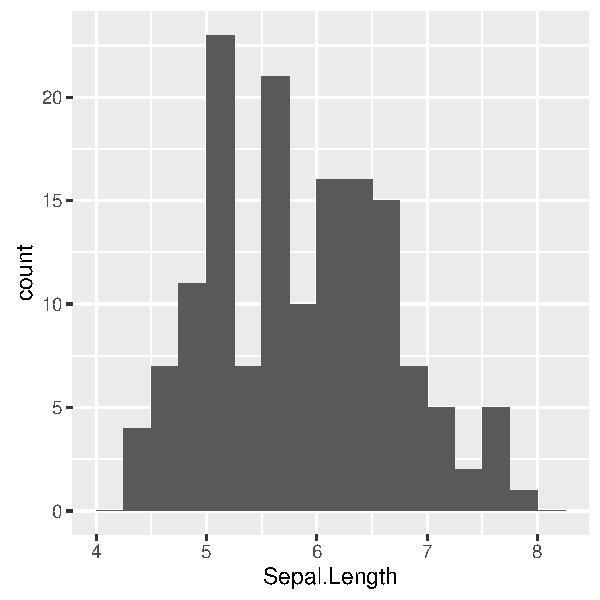
\includegraphics[width=\maxwidth]{figure/unnamed-chunk-2-1} 

\end{knitrout}

The above code indicates that we are using the \texttt{iris} dataset that is built in to R, we want to graph the \texttt{Sepal.Length} variable from those data, and we want a histogram so we use the \texttt{geom\_histogram}. When we want a different kind of graph of the same data, we just change the geom:

\begin{knitrout}
\definecolor{shadecolor}{rgb}{0.969, 0.969, 0.969}\color{fgcolor}\begin{kframe}
\begin{alltt}
\hlkwd{ggplot}\hlstd{(iris)} \hlopt{+} \hlkwd{aes}\hlstd{(}\hlkwc{x} \hlstd{= Sepal.Length)} \hlopt{+} \hlkwd{geom_density}\hlstd{()}
\end{alltt}
\end{kframe}
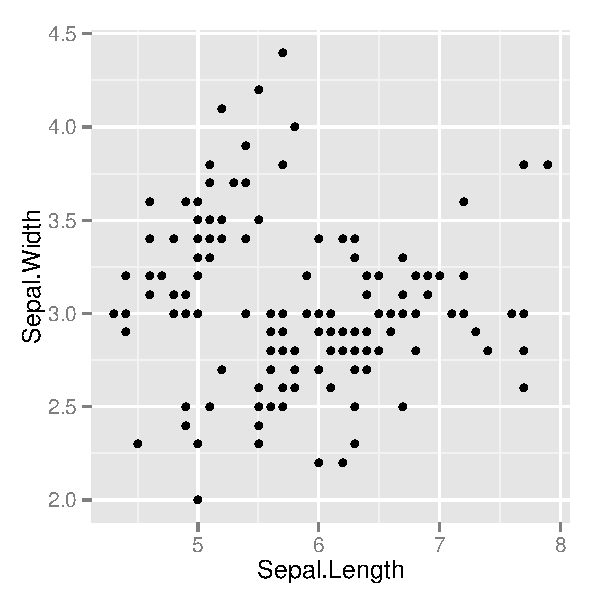
\includegraphics[width=\maxwidth]{figure/unnamed-chunk-3-1} 

\end{knitrout}

There are many, many geoms for single-variable plots (see the cheatsheet) and many, many more for two or more variable situations. Here's an example of a two-variable plot in ggplot2:

\begin{knitrout}
\definecolor{shadecolor}{rgb}{0.969, 0.969, 0.969}\color{fgcolor}\begin{kframe}
\begin{alltt}
\hlkwd{ggplot}\hlstd{(iris)} \hlopt{+} \hlkwd{aes}\hlstd{(}\hlkwc{x} \hlstd{= Sepal.Length,} \hlkwc{y} \hlstd{= Sepal.Width)} \hlopt{+} \hlkwd{geom_point}\hlstd{()}
\end{alltt}
\end{kframe}
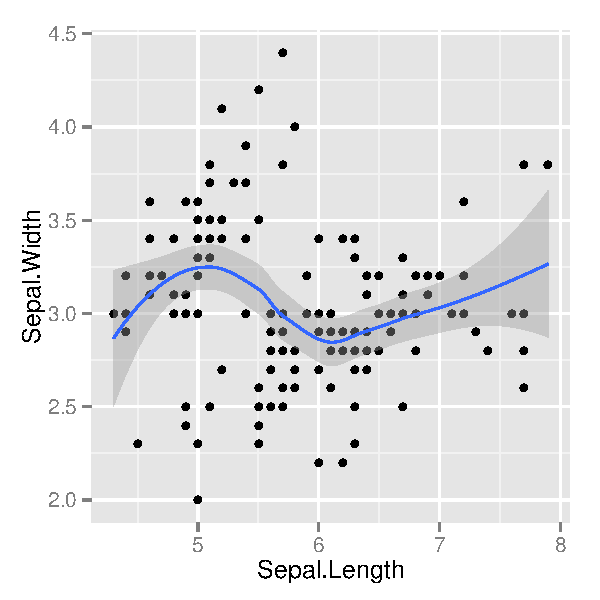
\includegraphics[width=\maxwidth]{figure/unnamed-chunk-4-1} 

\end{knitrout}

The neat feature of ggplot2 is that we can \textit{layer} multiple graphical elements on top of one another. So, in the above graph, we can easily add a smoothed line showing the relationship between the two variables more clearly:


\begin{knitrout}
\definecolor{shadecolor}{rgb}{0.969, 0.969, 0.969}\color{fgcolor}\begin{kframe}
\begin{alltt}
\hlkwd{ggplot}\hlstd{(iris)} \hlopt{+} \hlkwd{aes}\hlstd{(}\hlkwc{x} \hlstd{= Sepal.Length,} \hlkwc{y} \hlstd{= Sepal.Width)} \hlopt{+} \hlkwd{geom_point}\hlstd{()} \hlopt{+} \hlkwd{geom_smooth}\hlstd{()}
\end{alltt}
\end{kframe}
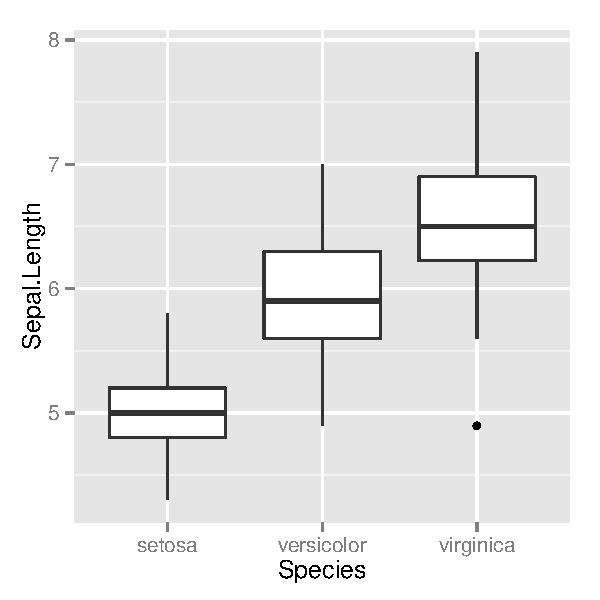
\includegraphics[width=\maxwidth]{figure/unnamed-chunk-5-1} 

\end{knitrout}


To display categorical data, we would use different geoms. Here we display boxplots showing the distribution of \texttt{Sepal.Length} across the different species in the \texttt{iris} dataset:

\begin{knitrout}
\definecolor{shadecolor}{rgb}{0.969, 0.969, 0.969}\color{fgcolor}\begin{kframe}
\begin{alltt}
\hlkwd{ggplot}\hlstd{(iris)} \hlopt{+} \hlkwd{aes}\hlstd{(}\hlkwc{x} \hlstd{= Species,} \hlkwc{y} \hlstd{= Sepal.Length)} \hlopt{+} \hlkwd{geom_boxplot}\hlstd{()}
\end{alltt}
\end{kframe}
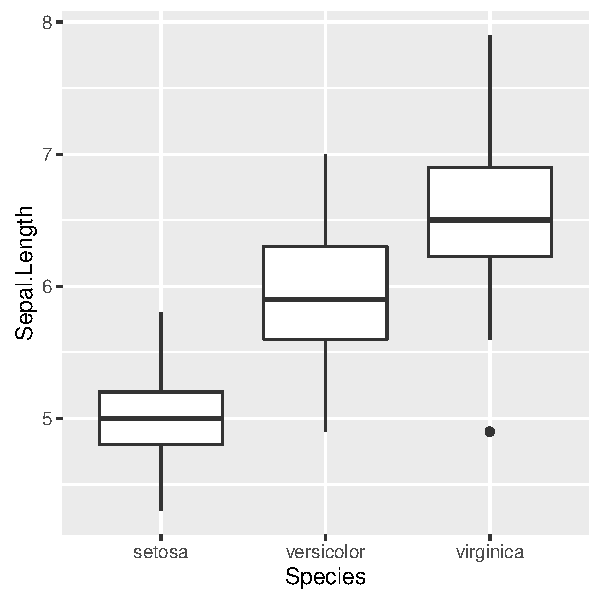
\includegraphics[width=\maxwidth]{figure/unnamed-chunk-6-1} 

\end{knitrout}



\subsection{Saving Plots}
Once you have created a plot, you will likely want to save it outside of R (for example, to include in a problem set). The easiest way to do this is by writing a \texttt{ggsave()} line into your code:

\begin{verbatim}
ggplot(iris) + aes(x = Species, y = Sepal.Length) + geom_boxplot()
ggsave("myplot.png")
\end{verbatim}

\noindent This saves your plot as a PNG file in your working directory.

\section{Basic Programming Tools: Logics, etc.}\label{sec:programming}
As I've stated above, R is a programming language. Thus, it will be helpful to understand some basic programming to help you move beyond the relatively simple tasks we've learned about so far. I will focus on four areas:
\begin{enumerate*}
\item Logicals
\item Functions
\item Apply
\item Loops
\end{enumerate*}

\subsection{Logicals}
Logicals allow you to test the equivalence of different R objects in any typical mathematical fashion:
\begin{itemize*}
\item Equal to: \texttt{==} \footnote{Note the double-plus (==), not to be confused with the single-plus (=), which is used to store a value.}
\item Greater than: \texttt{>}
\item Less than: \texttt{<}
\item Greater than or equal to: \texttt{>=}
\item Less than or equal to: \texttt{<=}
\item Not: \texttt{!}
\end{itemize*}
So, we can use these to produce \texttt{TRUE} or \texttt{FALSE} results from R, which is helpful when building complex programs. Generally it is not terribly helpful to test a simple logical like \texttt{2>1}, so instead these logical statements are often used as conditions for performing further operations inside an \texttt{if()} statement.

\subsubsection{IF-THEN, ELSE}
Logicals on their own, are not that helpful. Rather, they are helpful for building complex programs with subroutines that are only run under particular conditions. We could, for instance, set the value of one variable depending on the value of another, or only conduct an operation on an object if it is non-missing. While some programming languages require you to type ``then'' in order to actually execute the second part of an if-statement, R does not require this. Take a look at the following simple examples:

\begin{knitrout}
\definecolor{shadecolor}{rgb}{0.969, 0.969, 0.969}\color{fgcolor}\begin{kframe}
\begin{alltt}
\hlstd{x} \hlkwb{<-} \hlnum{2}
\hlkwa{if} \hlstd{(x}\hlopt{==}\hlnum{1}\hlstd{) q} \hlkwb{<-} \hlstr{"FAIL"}
\hlkwa{if} \hlstd{(x}\hlopt{==}\hlnum{2}\hlstd{) q} \hlkwb{<-} \hlstr{"SUCCESS"}
\hlstd{q}
\end{alltt}
\begin{verbatim}
## [1] "SUCCESS"
\end{verbatim}
\begin{alltt}
\hlkwa{if} \hlstd{(}\hlkwd{is.na}\hlstd{(x)) q} \hlkwb{<-} \hlstr{"FAIL"}
\hlkwa{if} \hlstd{(}\hlopt{!}\hlkwd{is.na}\hlstd{(x)) q} \hlkwb{<-} \hlstr{"SUCCESS"}
\hlstd{q}
\end{alltt}
\begin{verbatim}
## [1] "SUCCESS"
\end{verbatim}
\end{kframe}
\end{knitrout}

These logicals can also be combined with the AND \texttt{\&} or OR \texttt{\}} operators to produce logicals that meet more than one criterion.

\begin{knitrout}
\definecolor{shadecolor}{rgb}{0.969, 0.969, 0.969}\color{fgcolor}\begin{kframe}
\begin{alltt}
\hlstd{x} \hlkwb{<-} \hlnum{2}
\hlstd{q} \hlkwb{<-} \hlnum{NA}
\hlkwa{if} \hlstd{(}\hlopt{!}\hlkwd{is.na}\hlstd{(x)} \hlopt{&} \hlstd{x}\hlopt{>}\hlnum{2}\hlstd{) q} \hlkwb{<-} \hlstr{"SUCCESS"}
\hlstd{q}
\end{alltt}
\begin{verbatim}
## [1] NA
\end{verbatim}
\begin{alltt}
\hlkwa{if} \hlstd{(}\hlopt{!}\hlkwd{is.na}\hlstd{(x)} \hlopt{|} \hlstd{x}\hlopt{>}\hlnum{2}\hlstd{) q} \hlkwb{<-} \hlstr{"SUCCESS"}
\hlstd{q}
\end{alltt}
\begin{verbatim}
## [1] "SUCCESS"
\end{verbatim}
\end{kframe}
\end{knitrout}
Here we can see \texttt{q} is not set to equal \texttt{SUCCESS} under the first statement because while x is non-missing, x is not greater than 2. Under the second statement, however, where we use the OR operator \texttt{q} is set to \texttt{SUCCCESS} because x is non-missing, so it does not matter what the value of x is --- only one of the two logicals in parentheses needs to be true.

While we can string an infinitely long string of \texttt{if()} statements in a row, sometimes we do not need R to evaluate all of the statements --- for example, we may want to stop evaluating the \texttt{if()} statements once one of them is satisfied. We can use the \texttt{else if ()} and \texttt{else} commands in these instances.

\begin{knitrout}
\definecolor{shadecolor}{rgb}{0.969, 0.969, 0.969}\color{fgcolor}\begin{kframe}
\begin{alltt}
\hlstd{a} \hlkwb{<-} \hlnum{4}
\hlkwa{if} \hlstd{(a}\hlopt{==}\hlnum{1}\hlstd{) x}\hlkwb{=}\hlstr{"Stopped at 1"} \hlkwa{else}
\hlkwa{if} \hlstd{(a}\hlopt{==}\hlnum{2}\hlstd{) x}\hlkwb{=}\hlstr{"Stopped at 2"} \hlkwa{else}
\hlkwa{if} \hlstd{(a}\hlopt{==}\hlnum{3}\hlstd{) x}\hlkwb{=}\hlstr{"Stopped at 3"} \hlkwa{else}
\hlkwa{if} \hlstd{(a}\hlopt{==}\hlnum{4}\hlstd{) x}\hlkwb{=}\hlstr{"Stopped at 4"} \hlkwa{else}
\hlkwa{if} \hlstd{(a}\hlopt{==}\hlnum{5}\hlstd{) x}\hlkwb{=}\hlstr{"Stopped at 5"} \hlkwa{else}
\hlkwa{if} \hlstd{(a}\hlopt{==}\hlnum{6}\hlstd{) x}\hlkwb{=}\hlstr{"Stopped at 6 or larger"}
\hlstd{x}
\end{alltt}
\begin{verbatim}
## [1] "Stopped at 4"
\end{verbatim}
\end{kframe}
\end{knitrout}
You can see here that even though we had two lines of code after the:
\begin{verbatim}
if (a==4) x <- "Stopped at 4" else
\end{verbatim}
command, those lines were not evaluated because \texttt{a} was set to 4. Thus, we don't have to spend computing time and power to produce a logical \texttt{TRUE} or \texttt{FALSE} for each if-statement, only for the relevant if-statement.

\subsection{Functions}
While R and its supplemental packages provide an enormous amount of functionality, you sometimes feel compelled to write additional functionality to serve a particular need. In this case, you'll need to use the \texttt{function()} command. Let's say, for instance, that we had calculated daily high temperatures for a week in Fahrenheit, but needed them in Celsius. We could perform the conversion manually on each score:

\begin{knitrout}
\definecolor{shadecolor}{rgb}{0.969, 0.969, 0.969}\color{fgcolor}\begin{kframe}
\begin{alltt}
\hlstd{temp1.f} \hlkwb{<-} \hlnum{65}
\hlstd{temp1.c} \hlkwb{<-} \hlstd{((}\hlnum{65}\hlopt{-}\hlnum{35}\hlstd{)}\hlopt{*}\hlnum{5}\hlstd{)}\hlopt{/}\hlnum{9}
\hlstd{temp1.c}
\end{alltt}
\begin{verbatim}
## [1] 16.66667
\end{verbatim}
\end{kframe}
\end{knitrout}

Or we write a function to conduct the conversion without having to retype the math for each score:

\begin{knitrout}
\definecolor{shadecolor}{rgb}{0.969, 0.969, 0.969}\color{fgcolor}\begin{kframe}
\begin{alltt}
\hlstd{temps} \hlkwb{<-} \hlkwd{c}\hlstd{(}\hlnum{65}\hlstd{,}\hlnum{68}\hlstd{,}\hlnum{72}\hlstd{,}\hlnum{76}\hlstd{,}\hlnum{69}\hlstd{,}\hlnum{78}\hlstd{,}\hlnum{68}\hlstd{)}
\hlstd{ftoc} \hlkwb{<-} \hlkwa{function}\hlstd{(}\hlkwc{f}\hlstd{) \{}
        \hlstd{c} \hlkwb{<-} \hlstd{((f}\hlopt{-}\hlnum{35}\hlstd{)}\hlopt{*}\hlnum{5}\hlstd{)}\hlopt{/}\hlnum{9}
        \hlkwd{print}\hlstd{(c)}
\hlstd{\}}
\hlkwd{ftoc}\hlstd{(temps[}\hlnum{1}\hlstd{])}
\end{alltt}
\begin{verbatim}
## [1] 16.66667
\end{verbatim}
\end{kframe}
\end{knitrout}

\subsubsection{Apply}
This saves us a bit of time because it simplifies what we have to type, but it's still not very efficient. If we wanted to speed up the process even further, we could use R's \texttt{apply()} functions to automatically perform the function on every element in our \texttt{temps} vector.

\begin{knitrout}
\definecolor{shadecolor}{rgb}{0.969, 0.969, 0.969}\color{fgcolor}\begin{kframe}
\begin{alltt}
\hlstd{celsius} \hlkwb{<-} \hlkwd{sapply}\hlstd{(temps,}\hlkwc{FUN}\hlstd{=ftoc)}
\end{alltt}
\begin{verbatim}
## [1] 16.66667
## [1] 18.33333
## [1] 20.55556
## [1] 22.77778
## [1] 18.88889
## [1] 23.88889
## [1] 18.33333
\end{verbatim}
\begin{alltt}
\hlstd{celsius}
\end{alltt}
\begin{verbatim}
## [1] 16.66667 18.33333 20.55556 22.77778 18.88889 23.88889 18.33333
\end{verbatim}
\end{kframe}
\end{knitrout}
We can also use \texttt{apply()} built-in functions to matrices, vectors, and data.frames. This can be helpful if you want to calculate summary statistics for a number of different subgroups of observations within your dataset. Apply can also be used to do a lot of other things (including some cool and interesting things), but I won't go into the details here.

\subsection{Loops}
The last important piece of R programming that you should know about is looping. Like \texttt{apply()}, loops allow you to perform an otherwise tedious task a number of times on the same or different data, similar to using \texttt{apply()}. Loops and \texttt{apply()} are what really sets R apart from its competitors like SPSS, SAS, and Stata. There are several different types of loops that can be used, which are describe in detail at \url{http://cran.r-project.org/doc/manuals/R-lang.html#Looping}. The simplest loop can be used to perform the same temperature conversion we used above.

\begin{knitrout}
\definecolor{shadecolor}{rgb}{0.969, 0.969, 0.969}\color{fgcolor}\begin{kframe}
\begin{alltt}
\hlstd{celsius} \hlkwb{<-} \hlkwd{numeric}\hlstd{(}\hlkwd{length}\hlstd{(temps))}
\hlkwa{for} \hlstd{(i} \hlkwa{in} \hlnum{1}\hlopt{:}\hlkwd{length}\hlstd{(temps)) \{}
        \hlstd{celsius[i]} \hlkwb{<-} \hlstd{((temps[i]}\hlopt{-}\hlnum{35}\hlstd{)}\hlopt{*}\hlnum{5}\hlstd{)}\hlopt{/}\hlnum{9}
\hlstd{\}}
\hlstd{celsius}
\end{alltt}
\begin{verbatim}
## [1] 16.66667 18.33333 20.55556 22.77778 18.88889 23.88889 18.33333
\end{verbatim}
\end{kframe}
\end{knitrout}
Here, we tell R that we want to conduct a task for $i$ number of times, specified by 1 to the length of our \texttt{temps} vector. For each iteration of the loop, we take the $i^{th}$ element of the \texttt{temps} vector, perform the temperature conversion calculation and store the resulting value in the $i^{th}$ element of the \texttt{celsius} vector. When the loop completes, R displays nothing, so we have to call the \texttt{celsius} vector. If we didn't need to store each converted value, we could also use the \texttt{print()} command to simply display the resulting calculations like so:

\begin{knitrout}
\definecolor{shadecolor}{rgb}{0.969, 0.969, 0.969}\color{fgcolor}\begin{kframe}
\begin{alltt}
\hlkwa{for} \hlstd{(i} \hlkwa{in} \hlnum{1}\hlopt{:}\hlkwd{length}\hlstd{(temps)) \{}
        \hlkwd{print}\hlstd{(((temps[i]}\hlopt{-}\hlnum{35}\hlstd{)}\hlopt{*}\hlnum{5}\hlstd{)}\hlopt{/}\hlnum{9}\hlstd{)}
\hlstd{\}}
\end{alltt}
\begin{verbatim}
## [1] 16.66667
## [1] 18.33333
## [1] 20.55556
## [1] 22.77778
## [1] 18.88889
## [1] 23.88889
## [1] 18.33333
\end{verbatim}
\end{kframe}
\end{knitrout}
The \texttt{print()} function will be helpful if you run very large or complicated loops.

But now we've seen multiple ways to apply functions to objects. Which should we use in which situation? Given that we have nearly unlimited computing power and time, the distinctions between these methods are fairly small. \texttt{apply()} functions tend to be faster than loops, but that only matters if the task you're performing is very complicated. Loops are more versatile because you can perform multiple tasks within a single iteration of a loop, as well as nest loops inside one another. For example, if you needed to perform a task on each element of an $i$-by-$j$ matrix, you could nest a loop indexed by $j$ within a loop indexed by $i$, or vice versa. The final choice of how to program depends on the needs of the particular task you're aiming to complete. Often there many, many ways to accomplish the same task, which makes R uniquely versatile among statistical packages.

\section{Conclusion}\label{sec:conclusion}
So now you've learned the basic information you need to know to use R for this class. Hopefully this tutorial has helped you be less intimidated by and frustrated with the language and this course as a whole. Best of luck and let me know if you have questions!

\end{document}
